\documentclass[main]{subfiles}

\begin{document}
In {\it Normal Mode} the device samples analog signals, applies elliptical 
compensation, calculates angular position, and generates quadrature encoder signals
(figure \ref{FIG_SIGNAL_FLOW}).

These tasks are performed as fast as possible, in order to sample the signals at
the highest possible rate and also to introduce the least possible jitter in the 
generation of the output signals.

\begin{figure}[h]
    \centering
    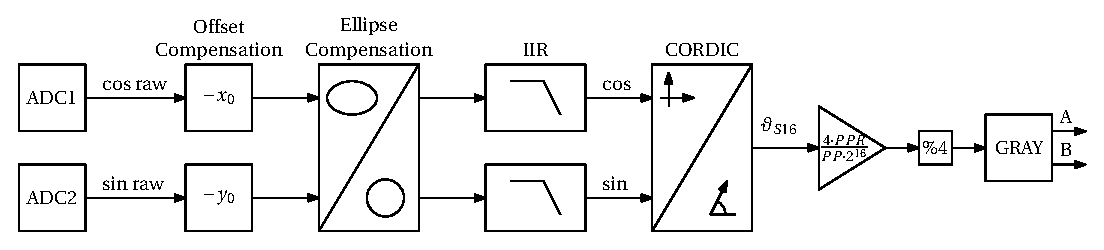
\includegraphics[width=\linewidth]{img/fw_norm_mode_sig_flow.eps}
    \caption{Signal Flow from analog measure to quadrature ancoder output}
    \label{FIG_SIGNAL_FLOW}
\end{figure}

As it can be seen in figure \ref{FIG_SIGNAL_FLOW}, after the analog measures 
have been acquired, some compensation operations are perfomed, in order to correct
some mechanical tolerances and production non-idealities.
The compensation consist of a constant offset subtraction (\ref{EQ_OS_COMP}), 
and a matrix product (\ref{EQ_ELL_COMP}).

\begin{equation}
    \begin{cases}
        cos_{os}(\vartheta) = cos_{raw}(\vartheta) - x_0\\
        sin_{os}(\vartheta) = sin_{raw}(\vartheta) - y_0
    \end{cases}
    \label{EQ_OS_COMP}
\end{equation}

\begin{equation}
    \begin{bmatrix}
        cos(\vartheta)\\
        sin(\vartheta)
    \end{bmatrix}=
    \begin{bmatrix}
        T_{00} & T_{01}\\
        T_{10} & T_{11}
    \end{bmatrix}
    \begin{bmatrix}
        cos_{os}(\vartheta)\\
        sin_{os}(\vartheta)
    \end{bmatrix}
    \label{EQ_ELL_COMP}
\end{equation}

This compensation works under the hypotesis that the samples describe an ellipse
even if it is not centered at the origin, and that there isn't any higher order 
distortion.
Said that, the offset subtraction shifts the points to center the ellipse at the 
origin, while the matrix multiplication operates a rotation to align ellipse axis
to Cartesian axis, and a scaling along those axis to a the circle with the 
desired radius.

\begin{minipage}{\linewidth}
\begin{lstlisting}[caption=compensation code]
//read ADCs registers, remove offset and shift them to 
//run 32 bits filters
adc_reg_cos = (int32_t)(ADC1->JDR1 - 
                        PVARS.cal_coeff_v[CAL_COEFF_X0]) << 16;
adc_reg_sin = (int32_t)(ADC2->JDR1 - 
                        PVARS.cal_coeff_v[CAL_COEFF_Y0]) << 16;

adc_cos_comp = ((adc_reg_cos>>10) * 
                PVARS.cal_coeff_v[CAL_COEFF_T00] + 
                (adc_reg_sin>>10) * 
                PVARS.cal_coeff_v[CAL_COEFF_T01]);

adc_sin_comp = ((adc_reg_cos>>10) * 
                PVARS.cal_coeff_v[CAL_COEFF_T10] + 
                (adc_reg_sin>>10) * 
                PVARS.cal_coeff_v[CAL_COEFF_T11]);
\end{lstlisting}
\end{minipage}

After that, the compensated values are passed through an IIR Low Pass filter
to remove some noise before phase calculation, and than they are loaded inside 
the cordic input register.

\begin{minipage}{\linewidth}
\begin{lstlisting}[caption=sin and cos filtering code]
//----------------------------------------------------------------
//                          Sin Cos Filter
//----------------------------------------------------------------
//
//                            1 - 1011/1024
//               H(z) = ------------------------------
//                         1  -  (1011/1024) z^-1
//
// alpha    = 1011/1024
// @Fs = 300kHz
// Ts       = 3.33us
// tau      = Ts/(1-alpha) = 263us approx
// fc       = 605 Hz approx
//----------------------------------------------------------------
adc_cos_filt_diff = (int32_t)(adc_cos_comp) - adc_cos_filt_state;
adc_cos_filt_state +=   (adc_cos_filt_diff >> 6) - 
                        (adc_cos_filt_diff >> 8) + 
                        (adc_cos_filt_diff >> 10);      
                        //fc = 600Hz @ 300kHz Fs
adc_cos_filt = (int32_t)(adc_cos_filt_state);

adc_sin_filt_diff = (int32_t)(adc_sin_comp) - adc_sin_filt_state;
adc_sin_filt_state +=   (adc_sin_filt_diff >> 6) - 
                        (adc_sin_filt_diff >> 8) + 
                        (adc_sin_filt_diff >> 10);      
                        //fc = 600Hz @ 300kHz Fs
adc_sin_filt = (int32_t)(adc_sin_filt_state);
\end{lstlisting}
\end{minipage}

The IIR filter is implemented with fixed point arithmetics, and using right 
shifts instead of divisions to keep it fast.

Considering that the developed sensor has
\begin{equation}
    \begin{cases}
        PP &= 4\\
        n_{max} &= 10 kRPM
    \end{cases}
\end{equation}

You can obtain the maximum sinewave signal frequency as 
\begin{equation}
    f_{max} = \frac{n_{max}}{60} \cdot PP = 667 Hz
\end{equation}

So the cutoff frequency has been set to 
\begin{equation}
    f_c \cong 600 Hz
\end{equation}

Since the sampling frequency is 
\begin{equation}
    f_s = 300 kHz
\end{equation}

the filter coefficient is found as follows
\begin{equation}
    \alpha = 1 - \frac{2\pi f_c}{f_s} \cong 0.9874
\end{equation}

Since we want to implement this coefficient using only shifts and sums we need 
to express $1-\alpha$ as a sum of negative-exponent powers of 2.

In this case for example we can write it like follows
\begin{equation}
    1 - \alpha \cong 0.0126 \cong \frac{13}{1024} = \frac{16-4+1}{1024} = 2^{-6} - 2^{-8} + 2^{-10}
    \label{EQ_ALPHA_DECOMP}
\end{equation}

Then recalling the first order IIR filter equation
\begin{equation}
    Y(z) = \frac{1-\alpha}{1-\alpha z^{-1}}X(z)
\end{equation}

we can write the difference equation as follows
\begin{equation}
    y(n+1) = \alpha y(n) + (1-\alpha) x(n+1)
\end{equation}

which easily becomes

\begin{equation}
    y(n+1) = y(n) + (1-\alpha) \left[x(n+1)-y(n)\right]
\end{equation}

Said that, and considering (\ref{EQ_ALPHA_DECOMP}) we can write the filter 
update function as follows

\begin{eqnarray}
    Diff  =& x(n+1) - y(n)\\
    State(n+1) =& State(n) + Diff \cdot 2^{-6} - Diff \cdot 2^{-8} + Diff \cdot 2^{-10}
\end{eqnarray}
    
The filtered values are then loaded into the cordic input register, and the 
phase is calculated. 
The Cordic peripheral outputs the angle in an integer format, which can be 
interpreted as a signed fixed point (Q1.15) in the range $[-1.0,1.0)$ or as a 
signed 16 bit integer (S16) in the range $[-2^{15},2^{15}-1]$ or as an unsigned 
16 bit integer (U16) in the range $[0, 2^{16}-1]$.

The computation has been carried out using the unsigned integer interpretation. 
Looking at figure \ref{FIG_SIGNAL_FLOW}, you can see that after the phase 
calculation, a gain is applied to the angle.
This is to get period maximum value that matches $4$ times the output {\it PPR} 
of the application divided by the input {\it PP} of the sensor, that create the 
number of periods per revolution of the sinewaves.
In our case, since $PPR = 64$ and $PP = 4$, the scaling operation becomes

\begin{equation}
    \vartheta_{scaled} = \vartheta \cdot \frac{4 \cdot PPR}{2^{16}PP} = 
    \vartheta \cdot 2^{-10}
\end{equation}

After this operation, which can simply be implemented with a 10 bit shift to the
right, $\vartheta_{scaled}$ will be in the range $[0, 63]$.
Indeed since the input sinewaves have a $4x$ periodicity with respect to the mechanical
one, it is sufficient to produce a $16 PPR$ output signal from the measured phase,
to obtain a $64 PPR$ output signal with respect to the mechanical phase.
The output state can finally be obtained from the rest of the integer division 
by $4$ of $\vartheta_{scaled}$ value. 
Since an integer division by $4$ is equivalent to a 2 bit right shift, and the 
rest is given by the 2 shifted-out bits, the state number can be simply obtained 
taking the 2 least significant bits to the variable $\vartheta_{scaled}$, obtaining 
a number in the range $[0,3]$.

\begin{figure}[h]
    \centering
    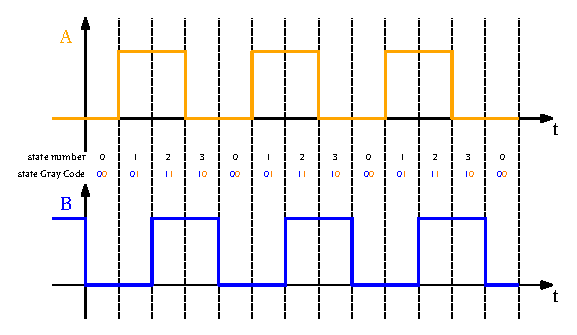
\includegraphics[width=\linewidth]{img/ab_signals.eps}
    \caption{Incremental encoder signals when rotating in positive direction}
    \label{FIG_AB_SIG}
\end{figure}

As can be seen in figure \ref{FIG_AB_SIG}, the outputs of incremental 
encoder signals cannot be generated by directly assigning the 2 bits of the 
calculated state variable, because we wouldnt obtain the correct switching sequence.
It is instead needed to convert the state variable into Gray Code using the 
table \ref{TAB_GRAY}. Then the least significant bit is assigned to signal {\it A},
while the most significant bit goes to signal {\it B}.

\begin{table}
    \centering
    \begin{tabular}{c|c}
        Number & Gray Code \\
        \hline
        0 & 00 \\
        1 & 01 \\
        2 & 11 \\
        3 & 10 
    \end{tabular}
    \caption{Gray Code conversion table}
    \label{TAB_GRAY}
\end{table}

Since it is unavoidable to have noise on measures, it is necessary to implement 
a deglitch operation, to avoid spurious commutations around the state switching 
instant.
To do so first the speed has been computed as filtered derivative of phase, and 
then, its sign has been used as rotating direction.

The filter applied to the speed, is similar to the {\it IIR} used for sampled 
values.
Here for simplicity the filter constant is defined as 

\begin{equation}
    \alpha = \frac{1023}{1024}
\end{equation}

which leads to a cutoff frequency of

\begin{equation}
    f_c = \frac{f_s(1-\alpha)}{2\pi} \cong 47 Hz
\end{equation}

In this case the difference equation is simpler 
\begin{eqnarray}
    Diff  =& x(n+1) - y(n)\\
    State(n+1) =& State(n) + Diff \cdot 2^{-10}
\end{eqnarray}

The derivative is calculated as
\begin{equation}
    speed = IIR(\vartheta(n) - \vartheta(n-1))
\end{equation}

\begin{figure}[h]
    \centering
    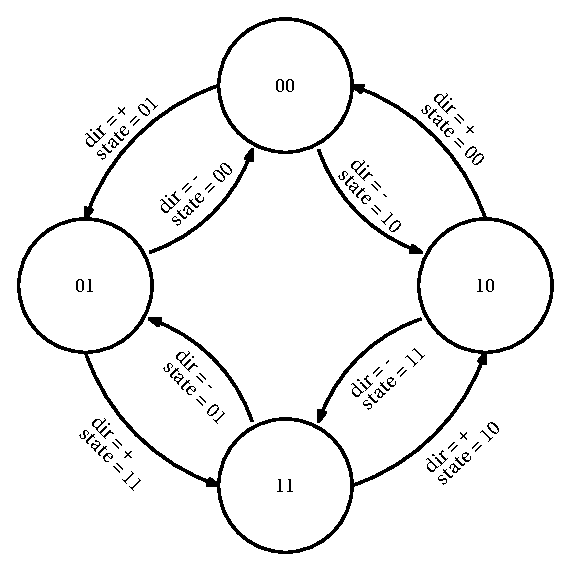
\includegraphics[width=0.6\linewidth]{img/state_change_fsm.eps}
    \caption{State change FSM}
    \label{FIG_STATE_FSM}
\end{figure}

Since the derivative is not divided by the sampling time (for faster computation), 
and since the angle is expressed to have $2^16-1$ matching the whole revolution,
the speed (measured in $Hz$ or $RPS$) will be expressed as 

\begin{equation}
    f_{mech} = \frac{speed}{2^{16}}f_s
\end{equation}

Then the deglitch action is carried out using a FSM like the one represented in 
figure \ref{FIG_STATE_FSM}, where an output state change is completed only if the 
calculated state is the state following the current one, considering the current 
direction.
Doing this you avoid multiple commutations when the noisy measured phase 
oscillates around the boundary between 2 states.

In order to avoid conditional statements and so have a lower and deterministic 
code execution time, this finite state machine is implemented as a 3d lookup 
table in the code (listing \ref{CODE_STATE_LUT}), where the inputs are direction, 
current state and the proposed next state. 
The output is the deglitched next state.

\begin{minipage}{\linewidth}
\begin{lstlisting}[caption=sin and cos filtering code,label=CODE_STATE_LUT]
    //state_lut[actual_dir][actual_state][proposed_next_state]
    __attribute__((section(".ccm_rodata")))
    const uint8_t state_lut[3][4][4] = 
    {
        //negative dir
        {  
            {0,0,0,3},
            {0,1,1,1},
            {2,1,2,2},
            {3,3,2,3}
        },
        //0 speed
        {
            {0,0,0,0},
            {1,1,1,1},
            {2,2,2,2},
            {3,3,3,3}
        },
        //positive dir
        {
            {0,1,0,0},
            {1,1,2,1},
            {2,2,2,3},
            {0,3,3,3}
        }
    }; 
\end{lstlisting}
\end{minipage}

The timings of the normal mode code execution, which are shown in figure 
\ref{FIG_TIMEBASE_NORMAL_MODE}, are handled with some interrupts.
Initially the ADCs are triggered by the {\it UIF (Update Interrupt)} of a hardware
timer at a frequency of $300 kHz$.
After the conversion has been completed (about $1.86\mu s$), one of the ADCs 
(both ADCs will finish their conversion at the same time, because they have same 
settings), triggers an {\it IRQ (Interrupt Request)}. Inside the {\it ISR 
(Interrupt Service Routine)}, the compensation and the filters are applied to the
sampled signals. Than signals are loaded into the Cordic input register, and the 
phase computation is automatically started.
When the phase data is ready, the peripheral triggers another {\it IRQ}.
Inside this {\it ISR}, the phase is read and all the computation to obtain 
{\it A} and {\it B} signals are performed. Finally the GPIOs are updated with the 
correct values, and the CPU goes in Idle state waiting for the next ADC {\it IRQ}.

The execution time of the whole algorithm is about

\begin{equation}
    T_{comp} = 1.36\mu s
\end{equation}

Leading to a CPU Load of

\begin{equation}
    CPU_{LD} = T_{comp} \cdot f_s = 40.8\%
\end{equation}

So we can state that the upper limit for the sampling rate is given by the ADCs
sampling time and not by the computation time; and the absolute maximum sampling 
rate is given by

\begin{equation}
    f_{s,max} = \frac{1}{1.86\mu s} \cong 538 kHz
\end{equation}

\begin{figure}[h]
    \centering
    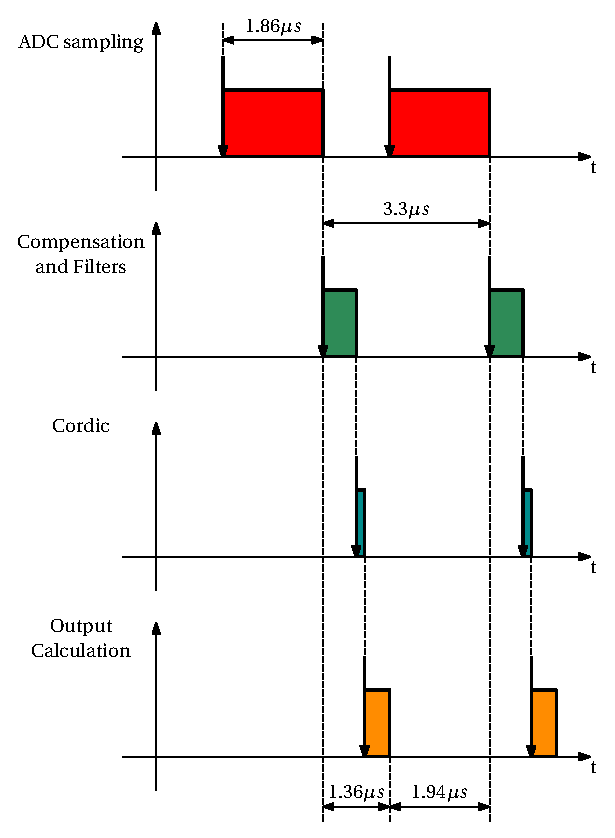
\includegraphics[width=0.6\linewidth]{img/timebase_norm_mode.eps}
    \caption{Timings of normal mode code execution}
    \label{FIG_TIMEBASE_NORMAL_MODE}
\end{figure}

With an output update like this, the output signal can only switch their states at
well defined discrete time instants, causing some jitter on the quadrature signals
edges, which could introduce phase errors, especially at high angular speeds.

To reduce the jitter, a {\it OneShot Mode} has been introduced.
To do so, together with the state, also the difference with next state is computed.
This value is then divided by the speed (already calculated), to obtain the time

\end{document}